\subsection{Regression}
Let's start from supervised learning. Supervised learning is a widely used approach when the values of a function in a certain set of points are known and it is required to construct a function that approximates an unknown function with a sufficiently high quality. Suppose the set of pairs is given:
\begin{equation*}
	D = \{ x^i, y^i \}_{i = 1}^N
\end{equation*}
, where 
\begin{equation*}
y^i = f(x^i) + \epsilon
\end{equation*}

In other words, here is presented the set of function values in some nodes. In general case not important the dimension of $x$ and $y$. If a scalar function is considered, then the process naturally requires the construction of a scalar approximant. In the case when it is required to approximate a vector-valued function, we can construct an approximation for each individual component. That is why the previous relation for $y$ can be rewritten as:
\begin{equation*}
	f: A \rightarrow B, \quad A \in R^n, B \in R^m
\end{equation*}

For simplicity, let $n = 1$, $m = 1$, for the other cases the same way.
There are a lot of ways to build the approximation, for example using linear regression model or using more advanced techniques. For example, Linear regression model is:
\begin{equation}
	\label{eq:linear_1d}
	\hat{y}^j = \beta_0 + \sum_{i = 1}^n \beta_i x^j_i = \beta_0 + \beta_1 x^j
\end{equation}
and the main goal is to estimate the coefficients $\beta_0$ and $\beta_1$. Here $n$ is the dimension of the $A$ space. If the dimension of $A$ is more than 1, the matrix form is more suitable for \eqref{eq:linear_1d}:
\begin{equation}
	\label{eq:linear_matrix_form}
	\hat{y}^j = \beta_0 + \sum_{i = 1}^n \beta_i x^j_i = x^T \beta \implies Y = X \beta
\end{equation}
In the general case, \eqref{eq:linear_matrix_form} can be rewritten as:
\begin{equation}
	\label{eq:linear_expansion}
	\hat{y}^j = \beta_0 + \sum_{i = 1}^K \beta_i \phi_i(x^j_i) \quad \text{or} \quad Y = Z \beta, \text{where } Z^j_i = \phi_i(x^j_i)
\end{equation}
, where the functions $\phi_j$ are predefined earlier and depend on the specifics of the problem. $ K $ is the number of predefined functions.

To estimate the unknown coefficients in the problem, it is necessary to determine a quality function characterizing the quality of the approximation of the initial data. This function is called the residual or the quality function, or the loss function:
\begin{equation}
	R(x) = \hat{y} - y, \quad R(x^i) = R^i = \hat{y}^i - y^i
\end{equation}
Here $R^i$ is the residual or deviation at the point $x_i$, $\hat{y}^i$ is the value obtained from the approximating function.
residual at $x^i$.  The main goal is to minimize the sum of residuals:
\begin{equation*}
	\sum_{x^i \in X} R(x) \rightarrow min, \quad \text{or }  \sum_{x^i \in X} g(R(x)) \rightarrow min
\end{equation*}
, $g$ is monotonic 
function - loss function. This is important, because in a specific task or to justify the construction of the coefficient estimation process, it is sometimes more convenient to use not a sum of squares, but some transformation of this function.

The most widely used loss function for this type of problem is the mean squared error or $R^2$ score. In this work, the mean squared error will be used:
\begin{equation}
	\mathcal{L} = \dfrac{1}{N} \sqrt{\sum_{i = 1}^N \left ( y_i - \hat{y_i} \right )^2} = \dfrac{1}{N} \sqrt{\sum_{i = 1}^N \left ( R^i \right )^2}
	\label{eq:loss}
\end{equation}
where $y^i$ is the function value at $x^i$ from the set of known points and $\hat{y^i}$ predicted from the model.

To estimate the coefficients, the least squares method is applied to \eqref{eq:linear_matrix_form}:
\begin{equation*}
	\dfrac{\partial \mathcal{L}}{\partial \beta_i} = \dfrac{\partial}{\partial \beta_i} \dfrac{1}{N} \sqrt{\sum_{i = 1}^N \left ( R(x^i) \right )^2}
\end{equation*}

The considered method is very effective for estimating coefficients, for analysis and can be effectively solved using linear algebra tools. Using statistical methods, the number of necessary functions and their values are estimated with their confidence intervals. A problem may arise when the ability to calculate derivatives is absent or the extremum of the loss function is not unique.

\subsection{Regularization}
From \eqref{eq:linear_matrix_form} linear regression model is:
\begin{equation*}
	Y = X \beta
\end{equation*}
$\beta$ - unknown parameters. The residual for this model is also known. Now, just substitute the residual to loss function \eqref{eq:loss}:
\begin{equation*}
	\mathcal{L} = \dfrac{1}{N} \sqrt{\sum_{i = 1}^N \left ( R^i \right )^2} \Leftrightarrow \| Y - X \beta \|^2 \rightarrow min
\end{equation*}
\begin{equation}
	\| Y - X \beta \|^2 = \left ( Y - X \beta \right )^T \left ( Y - X \beta \right ) =  Y^T Y - Y^T X \beta - \beta^T X^T Y + \beta^T X^T X \beta
	\label{eq:linear_opt}
\end{equation}
And compute $\dfrac{\partial \mathcal{L}}{\partial \beta}$:
\begin{equation*}
	\dfrac{\partial }{\partial \beta} \left [ Y^T Y - Y^T X \beta - \beta^T X^T Y + \beta^T X^T X \beta \right ] \implies X^T Y =  X^T X \beta \\
	\beta = \left ( X^T X \right )^{-1} X^T Y
\end{equation*}

The last operation was very dangerous in the sense that the inverse matrix does not always exist or may be poorly conditioned. For example, if the determinant of the matrix $ X ^ T X $ does not exist, what should I do? Or is the matrix $X ^ T X$ poorly conditioned?
The answer is to use special methods to avoid this - regularization methods.
Look at the \eqref{eq:linear_opt} and add the additional term \cite{kress2012numerical}:
\begin{equation}
	\| Y - X \beta \|^2 + \lambda \| \beta \|^2 \implies \beta = \left ( X^T X + \lambda I \right )^{-1} X^T Y
\end{equation}
It follows from \cite{kress2012numerical} that $ X ^ T X + \lambda I $ is not a singular matrix and actually has a lower condition number than $ X ^ T X $. In addition, there are many regularization methods, some of which are \cite{ridge}, \cite{lasso}, \cite{dantzig_selector}, \cite{rlad}, \cite{slope}.
This is just one simple problem that may arise in the process of evaluating coefficients. By the way, there are more powerful methods to avoid some problems: random forest, gradient increase \cite{bishop}, neural networks \cite{haykin}.

As an example of the use of regularization, we can consider the simple problem of estimating a one-parameter model using different methods of regularization. Let $y = f(x) = k  x + \epsilon, k = 10$. At the fig. \ref{fig:regularizations} seen, that regularization impact is big. After applying linear models (\cite{ridge}, \cite{lasso}, \cite{rlad}) for this problem with different regularization methods was got a different results. The RLAD method estimate the $\hat{k} = 10.498$, Ridge method $\hat{k} = 9.109$ and Lasso - $\hat{k} = 9.604$. Results slightly different because the key difference is using different norms for regularization. It is an important fact for the next work, where more complex regression models will be used. 

\begin{figure}[h]
	\centering
	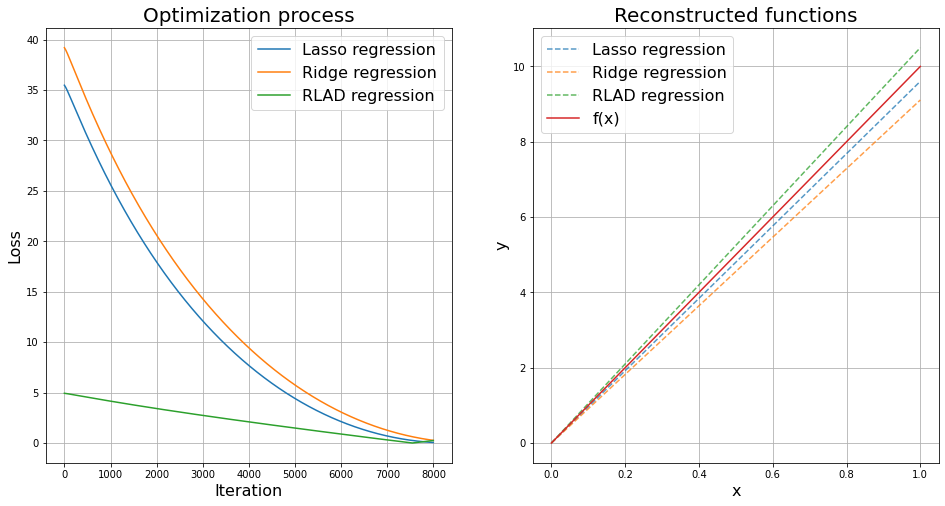
\includegraphics[width=\textwidth]{images/chapter2/reularization_impact.png}
	\caption{Comparison of different regularizations techniques}
	\label{fig:regularizations}
\end{figure}